\documentclass{report}

\usepackage{caption}

\title{XTetris: Official Report}
\author{Mirco De Zorzi \\ \texttt{<mircodezorzi@protonmail.com>}}
\date{}

\begin{document}

\maketitle

\section{Team Composition}

\begin{itemize}
  \item Mirco De Zorzi (mat. 891275).
\end{itemize}

\section{Project Structure}

\subsection{Toolkit}
\label{ssec:toolchain}

\begin{itemize}
  \item pre-commit: runs \texttt{clang-format}, \texttt{clang-tidy}, \texttt{oclint}, \texttt{uncrustify}, \texttt{cppcheck} and \texttt{cpplint} on commit to guarantee code consistency;
  \item Makefile: controls the generation of object files and executables;
  \item ccache: object caching to speed up re-compilation;
  \item gcc: compiler.
\end{itemize}

\subsection{Scaffolding Tools}

To generate the project scaffold \href{https://github.com/mircodezorzi/secretary}{\texttt{mircodezorzi/secretary}} was used. Running the following command will create a repository with all tools described in section \ref{ssec:toolchain}.

\begin{minted}[
  frame=single,
]{sh}
$ secretary create libdz --template c-make
\end{minted}

\subsection{\texttt{libdz} Architecture}

\texttt{libdz} uses a callback model for all event handling, from keyboard and mouse events, to button clicks. What follows is a minimal \textit{working} example of the high level API that the library exposes:

\begin{minted}[
  frame=single,
]{c}
void on_loop(engine_t* e) {
  // draw ...
}

void on_keyboard(engine_t* e, kb_ev_t ev) {
  // handle keyboard event ...
}

void on_mouse(engine_t *e, mouse_ev_t ev) {
  // handle mouse event ...
}

engine_t *e = engine_new(
  on_loop, on_mouse, on_keyboard);
engine_loop(e)
\end{minted}

\subsection{Multiplayer Implementation}

Multiplayer orchestration is handleed through a centralized server written in Go, and ideally running on a publicly reachable endpoint, such as a EC2\footnote{https://aws.amazon.com/ec2/} instance.
For demonstration porpuses only the game server is going to be run locally, along side the two clients.

\begin{figure}[h]
\centering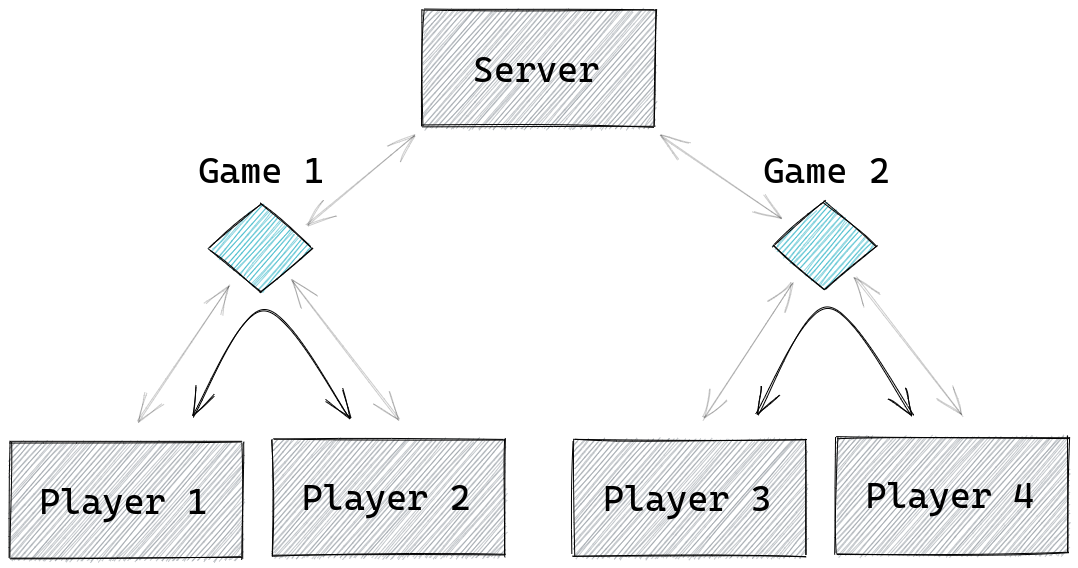
\includegraphics[width=0.45\textwidth]{infra.png}
\caption{Client-Server Model. Black arrows represent data flow from the client's prespective, while the gray ones represent what actually happens. \texttt{Game N} represents the abstracted data structure that holds the games's state.}
\end{figure}

\begin{listing}[h]
\begin{minted}[
  frame=single,
]{go}
type userConn struct {
	conn    net.Conn
	scanner *bufio.Scanner
	state   connState
	user    string
	field   []int
	room    string
}

type room struct {
	A *userConn
	B *userConn
}
\end{minted}
\caption{Simplified data structures used by the server. Refer to \texttt{server/main.go} for more context.}
\end{listing}

\section{Unimplemented Features}

Most of the issues listed below belong to a ever-growing list of TODOs of this project. Due to a series of time constraints (and lock of desire to do so) 

\begin{itemize}
  \item Cleanup project directories and source code.
  \item Rewrite makefiles to completely automate the build process.
  \item Both client-side and server-side authentication and session handling is somewhat brittle. In case one of the clients times-out, there is no way to recover a game session;
  \item The UI library (\texttt{libdz}) is still in a \textit{work-in-progess} state. Most components require a close-to-complete rewrite, and the code has yet to be hardened, so security is not guaranteed. Some missing features from the library are:
  \begin{itemize}
    \item non-blocking TCP client and server;
    \item scenes: state-machine management by the engine to automate navigation between them panels;
    \item panels, textboxes, checkboxes...: layout automation for complex menus (refer to \href{https://github.com/mircodezorzi/sym}{\texttt{mircodezorzi/sym}} for an close implementation);
    \item better bounding-box handling for all widgets: allow for a widget to have a \texttt{parent}, altering it's origin point in relation to the parent's one.;
    \item pass \texttt{context\_t*} to all callback functions instead of the parent object;
  \end{itemize}
  \item Better field state handling. Currently it is possible to send arbitrary information to the server, effectively making it possible to set one own's field to an arbitrary state. This would make cheating trivially simple.
  \item Add options menu to change field size, key bindings or multiplayer settings.
  \item The networking code is really badly written. It does not follow the ANSI standard and doesn't try to optimize anything.
  \item Player Vs. AI is missing.
  \item Thread safety in server is missing.
  \item In multiplayer mode when a player clears 4 rows with a single drop, the opponent's field should fill with \texttt{n} rows of ghost tetraminos (with one of the colmns empty). This has not been implemented yet (due to time constraints), although doing so would be trivial.
  \item A local/global scoreboard is missing.
  \item The option to view a list of active players is missing (and therefore a lobby system similar to other online multiplayer games).
  \item When, in multiplayer, a player dies, the oppont will be able to continue playing untill he loses. The losing opponent's field will be filled with red. \textbf{This is indeed a feature, and not a botch fix due to the lack of time to implement a real "game over" screen}.
  \item Rewrite this entire report, as it is abysmally unorganized and confused.
\end{itemize}

\noindent Refer to the source and header files for more documentation related to unimplemented features.

\end{document}
